\begin{comment}
Aufsetzen der Suche
\begin{itemize}
    \item Indizieren von ein bis zwei der untersuchten Medienformaten.
    \item Suchabfragen erstellen.
\end{itemize}

\paragraph{Result} \hfill \\
\begin{itemize}
    \item Ein lauffähige Instanz von Lucene.
    \item Vorbereitung der Dokumente (Mediadateinen) um die Metadaten zu extrahieren.
\end{itemize}
\end{comment}


\chapter{Information Retrieval}
\label{ch:setup}

Im vorigen Kapitel haben wir uns die Metadaten der
zu indizierenden Dokumente angeschaut. Diese Metadaten
werden wir nun mit der Library Apache Lucene \cite{web:lucene}
indizieren und durchsuchen.

\begin{figure}[ht]
    \centering
    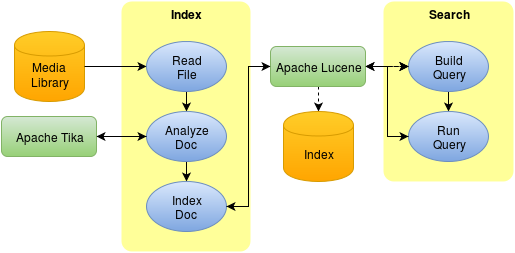
\includegraphics[width=\textwidth]{architecture-tika-lucene}
    \caption{Architektur Information Retrieval Applikation}
    \label{fig:tika-lucene}
\end{figure}

In \cref{fig:tika-lucene} sehen wir die einzelnen Elemente
welche in einer Information Retrieval Applikation mitwirken
und in welchen Schritte welche Apache Libraries verwendet
werden.
Aus dieser Übersicht wollen wir uns nun dem letzten Schritt des Erstellens
des Index zuwenden, dem Indizieren der Metadaten der Dokumente.
\cite{web:tika-lucene}

\section{Index erstellen}
\label{sec:createindex}
Die Metadaten, welche in \cref{sec:parse} gelesen
wurden, bilden pro gelesene Datei eine Menge von
Attributen mit Werten. Aus einer solchen Menge
wählen wir die gewünschten Attribute aus und 
fassen diese zusammen zu Dokumenten. Diese Dokumente
werden dem Index hinzugefügt.

\paragraph{Shared Memory in Linux} \hfill \\
Zugriffe auf den Index sollten möglichst schnell
ausgeführt werden. Am schnellsten sind diese, wenn
sich der Index im Arbeitsspeicher befindet. Da auf
Linux Systemen standardmässig das Verzeichnis
Shared Memory \emph{/dev/shm} im Arbeitsspeicher
geladen wird, werden wir den Index darin erstellen.
Es ist anzumerken, dass Dateien in diesem Verzeichnis
verloren gehen wenn das System heruntergefahren
wird.\cite{web:shm}

In folgendem Listing betrachten wir die Funktion,
mit welcher wir aus dem \emph{fileName} und den
\emph{metadata} ein Dokument erstellen. Allenfalls
vorhandene \emph{keywords} fügen wir dem Dokument als
einzelne \emph{StringFields} hinzu. Ein \emph{StringField}
ist ein String welcher als ganzes indiziert wird.
Das \emph{TextField} wird bei Leerzeichen oder anderen
Trennzeichen gesplittet und als mehrere \emph{Strings}
indiziert. Mit dem \emph{boolean} Wert \emph{Store.YES}
sagen wir, dass der Wert des indizierten Attributes
auch abgelegt werden soll. Alle Attribute welche leer
sind werden nicht indiziert. Weiter werden alle Attribute
welche nicht explizit indiziert werden verworfen.

\begin{lstlisting}[style=myScalastyle]
def mkDocument (fileName:String, metadata:Metadata): Document = {

    val fieldPat = "([a-z0-9]+):([a-z0-9]+)".r
    val xmpdmAttrs = Array("album", "releasedate", "genre")
    val doc = new Document()
    doc.add(new StoredField("file", fileName))
    
    for (key <- metadata.names()) {
        val name = key.toLowerCase()
        val value = metadata.get(key)
        if (!StringUtils.isBlank(value)) {
            name match {
                case "keywords" => 
                    for (keyword <- value.split(",?(\\s+)")) {
                        doc.add(new StringField(name, keyword, Store.YES))
                    }
                case "title" | "author" | "composer" =>
                    doc.add(new TextField(name, value, Store.YES))
                case fieldPat("xmpdm", attr) if xmpdmAttrs contains attr =>
                    doc.add(new TextField(attr, value, Store.YES))
                case _ => ()
            }
        }
    }
    doc
}
\end{lstlisting}

In einem Loop iterieren wir nun rekursiv über alle
Dateien in der Media Library, erstellen zu jeder FLAC und MP3
Datei ein Dokument und fügen dieses Dokument zum Index
hinzu.

\paragraph{Rekursiv über Dateien Iterieren} wird mit der
\emph{listFiles} Methode aus dem Apache Package
\emph{org.apache.commons.io.FileUtils} ausgeführt.
Diese Methode erlaubt auf einfache Weise rekursiv
über alle Dateien eines Verzeichnisses zu iterieren.
\cite{web:fileutils}

\section{Abfragen ausführen}
Auf dem soeben erstellten Index führen wir nun eine Abfrage
aus. Die Abfrage soll über mehrere Attribute ausgeführt
werden.

Abfragen müssen der Lucene Query Parser Syntax entsprechen.
Damit können unter anderem Proximity Searches, Range Searches
oder Fuzzy Searches ausgeführt werden, es können
zu durchsuchende Attribute festgelegt werden oder
auch einzelne Terme
miteinander verknüpft werden. \cite{web:lucenesyntax}

Für unsere Abfrage wollen wir für das Erste nur 
nach einem Begriff in mehreren Attributen suchen.
Dazu müssen wir den \emph{MultiFieldQueryParser}
verwenden. Nachfolgend parsed der \emph{parser}
einen Abfrage String und gibt eine \emph{Query}
zurück. Diese Query \emph{q} übergeben wir dem
\emph{IndexSearcher}. Von dem \emph{collector}
werden danach die gefundendenen Resultate geholt.
\cite{web:lucenedoc,web:luceneintro}

\begin{lstlisting}[style=myScalastyle]
def apply() {
    
    val indexDir = Paths.get(Config.indexPath)
    val index = FSDirectory.open(indexDir)

    // Build a Query object
    val fields = Array("album", "author", "composer", "album", "title")
    val analyzer = new StandardAnalyzer()
    val parser = new MultiFieldQueryParser(fields, analyzer)

    Try(parser.parse("Shpongle")) match {
        case Success(q) => 
            val hitsPerPage = 10
            val reader = DirectoryReader.open(index)
            val searcher = new IndexSearcher(reader)
            val collector = TopScoreDocCollector.create(hitsPerPage)
            searcher.search(q, collector)
            
            println("total hits: " + collector.getTotalHits())
            val hits = collector.topDocs().scoreDocs
            for (hit <- hits) {
                val doc = reader.document(hit.doc)
                println(doc.get("file") + "  (" + hit.score + ")")
            }
        case Failure(e) => println(e.toString())
    }       
}
\end{lstlisting}

Wie wir nun gesehen haben, erlaubt einem die Apache
Lucene Library auf einfache Weise, aus Dokumenten
einen Index zu erstellen und an diesen Abfragen zu
stellen. Im nächsten Kapitel wollen wir den so erstellten
Index der Media Library etwas genauer betrachten.
